\par \indent In order to apply a multi-dimensional Gaussian filter to ``smooth''
the bold image, we use the SciPy module's \texttt{gaussian\_filter} function. 
We made this decision because convolution does not truncate the kernel. Using
zero padding, the points toward the edge get pulled down towards zero because
they are part-made of the results of taking the product of zeros with the kernel
values. We prefer using another method for working with the data off the image's
edge. [Figure \ref{fig:smoothing}]

\begin{figure}[!ht]
\centering
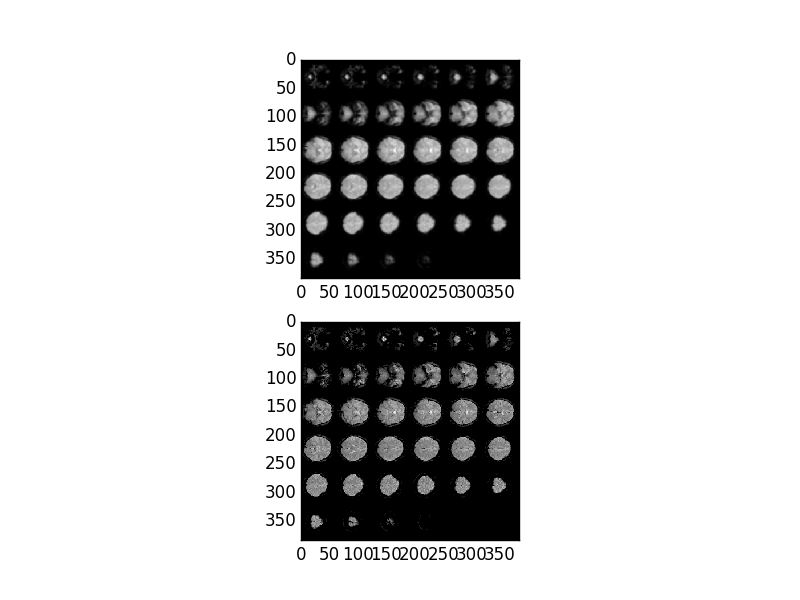
\includegraphics[width=120mm]{images/smooth_fig.png}
\caption{Compare two bold images before and after smoothing}
\label{fig:smoothing}
\end{figure}
